\chapter{Zadanie projektowe}

Zadaniem projektowym tej części naszej pracy było przygotowanie oraz dobranie optymalnych nastawów regulatorów w środowisku Matlab. W części a) należało dobrać strukturę i nastawy dwupętlowego układu regulacji PI/PID z odsprzęganiem i bez odsprzęgania. Kolejno, należało zaprojektować i zaimplementować analityczny regulator predykcyjny z uwzględnieniem ograniczeń przez rzutowanie oraz, w części c), numeryczny regulator predykcyjny z uwzględnieniem ograniczeń na sterowanie. Następnie należało porównać działanie tych regulatorów.
\\\\ Algorymem regulatora jaki należało zaimplementować w części b) i c) w ramach naszego zadania był regulator predykcyjny DMC (Dynamic Matrix Control)\\\\

\section{Regulacja DMC}
\begin{figure}[h!]
	\centering
	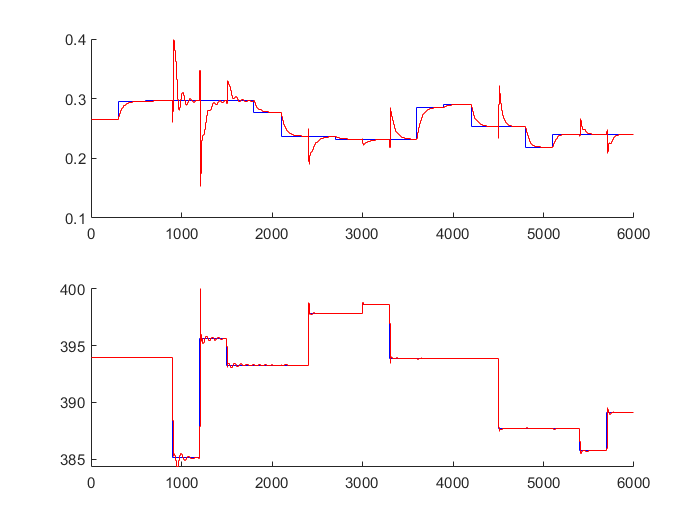
\includegraphics[width=.6\linewidth]{img/yDMC.png}
	\label{ch2:Zadanie}
	\caption{Regulacja DMC analityczna - wyjście na tle wartości zadanej}
\end{figure}
\begin{figure}[h!]
	\centering
	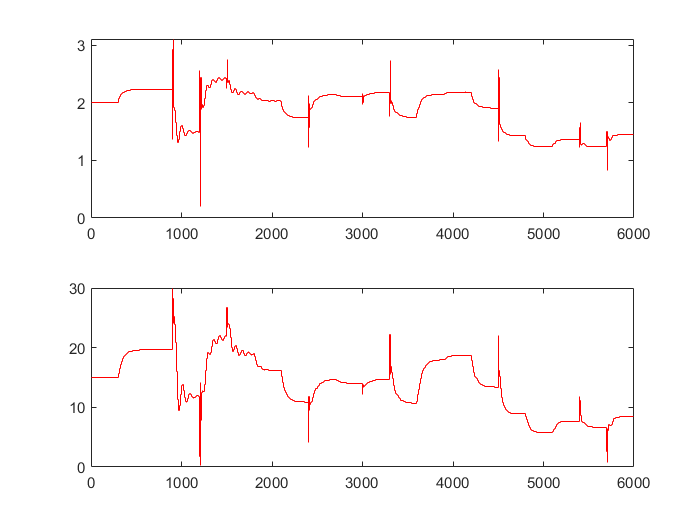
\includegraphics[width=.6\linewidth]{img/uDMC.png}
	\label{ch2:Zadanie}
	\caption{Regulacja DMC analityczna - sterowanie}
\end{figure}
\begin{figure}[h!]
	\centering
	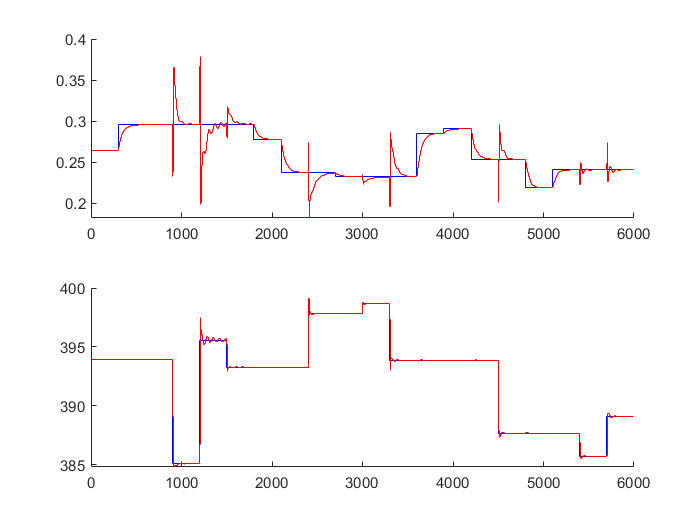
\includegraphics[width=.6\linewidth]{img/yDMCnum.png}
	\label{ch2:Zadanie}
	\caption{Regulacja DMC numeryczna - wyjście na tle wartości zadanej}
\end{figure}
\begin{figure}[h!]
	\centering
	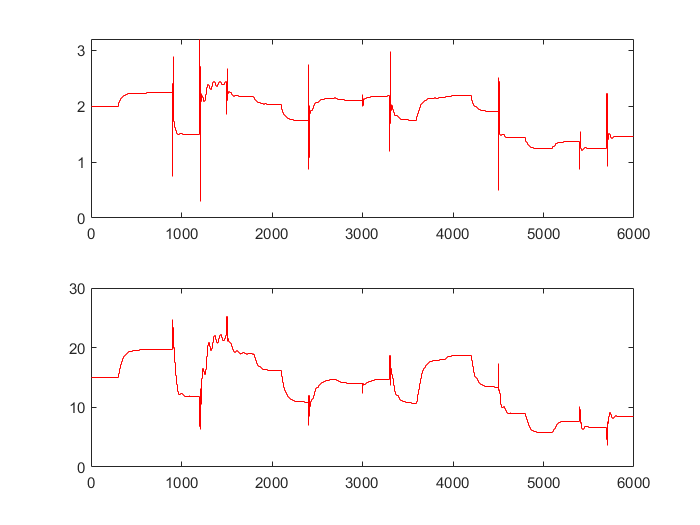
\includegraphics[width=.6\linewidth]{img/uDMCnum.png}
	\label{ch2:Zadanie}
	\caption{Regulacja DMC numeryczna - sterowanie}
\end{figure}
\newpage
Działanie prezentowanych powyżej algorytmów najłatwiej porównać będzie prezentując je na wspólnym rysunku. 
Zgodnie z oczekiwaniami, regulacja przebieg w podobny sposób dla obu implementacji regulatora. W obu przypadkach występują oscylacje wyjścia przy dużych skokach wartości zadanej dla wyjścia T procesu, dla niewielkich skoków wartości zadanej, regulatory porównywalnie szybko sprowadzają wartość wyjścia T do zadanego poziomu. Wyjście CA również zachowuje porównywaly przebied przy zastosowaniu regulatora analitycznego, czy numerycznego. Ta zmienna wyjściowa, nieco wrażliwsza w regulacji, a oba typy regulatorów spowodowały zbliżony, a często pokrywający się przebieg, z podobnymi wysokościami przeregulowań.
Należy jednak zaznaczyć, że mimo podobieństwa wyników i przebiegu sterowań, obliczenia dla algorytmu numerycznego trwały znacznie dłużej niż dla analitycznego.
\begin{figure}[h!]
	\centering
	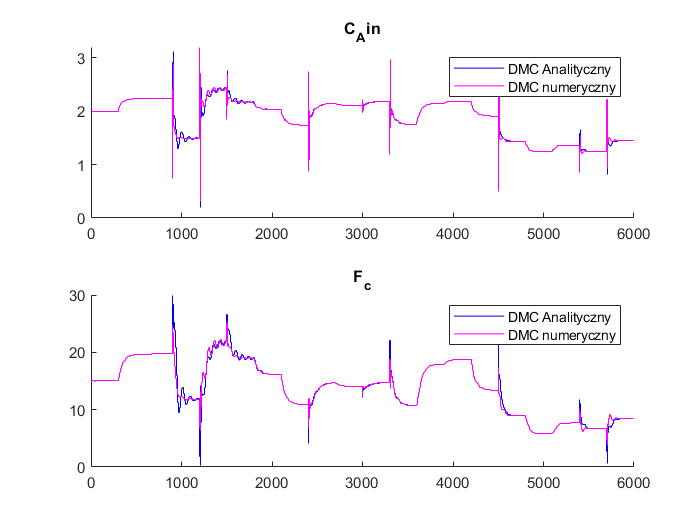
\includegraphics[width=.6\linewidth]{img/uComparedDMC.png}
	\label{ch2:Zadanie}
	\caption{Regulacja DMC analityczna i numeryczna - sterowanie}
\end{figure}
\begin{figure}[h!]
	\centering
	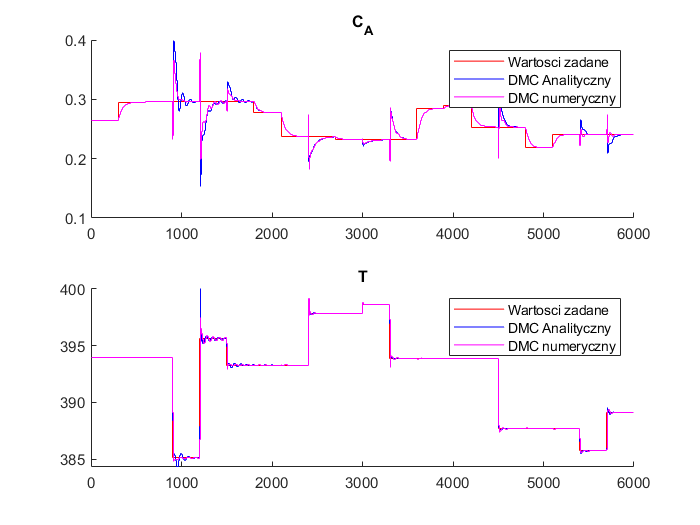
\includegraphics[width=.6\linewidth]{img/yComparedDMC.png}
	\label{ch2:Zadanie}
	\caption{Regulacja DMC analityczna i numeryczna - wyjścia}
\end{figure}